\section{Use case diagram}
\subsection{Points communs}
	Etant donné la nature des deux applications, de nombreux points communs sont à souligner dans les use cases comme les logs, gestion des notifications et gestion des paramètres.
\newline
\newline
	Concernant le système de log, cela peut s'apparenter à une application "classique" contenant des utilisateurs.
\newline
\newline
	Pour la gestion des notifications, l'utilisateur aura la possibilité de voir les détails des notifications qu'il aura reçu et il aura le choix de les accepter ou de les refuser. En plus de ça, l'utilisateur aura la possibilité de rafraichir la page pour voir apparaitre de nouvelles notifications (comme dit dans l'énoncé).
\newline
\newline
	En ce qui concerne la gestion de paramètre, l'utilisateur aura la possibilité de modifier son mot de passe en ayant reçu un mail de confirmation au préalable. Pour la gestion des langues, il aura le droit de changer la langue actuelle de l'application, d'en ajouter et d'en choisir une qui sera sa langue favorite.
\newline
\newline
	Nous pouvons observer que le serveur est un acteur qui enregistrera toutes les informations utiles. En plus de ça, il jouera le role de correspondant entre le client et le fournisseur par le biais du use case : "transférer les données".

\newpage

\subsection{Client}
	Tout d'abord, le client pourra gérer ses données de consommation par le biais de ses portefeuilles.
\newline
\newline
	Ensuite, nous pouvons souligner le fait que d'ajouter des contrats est indépendant du fait de créer un portefeuille. 

\begin{figure}[h]
\centering
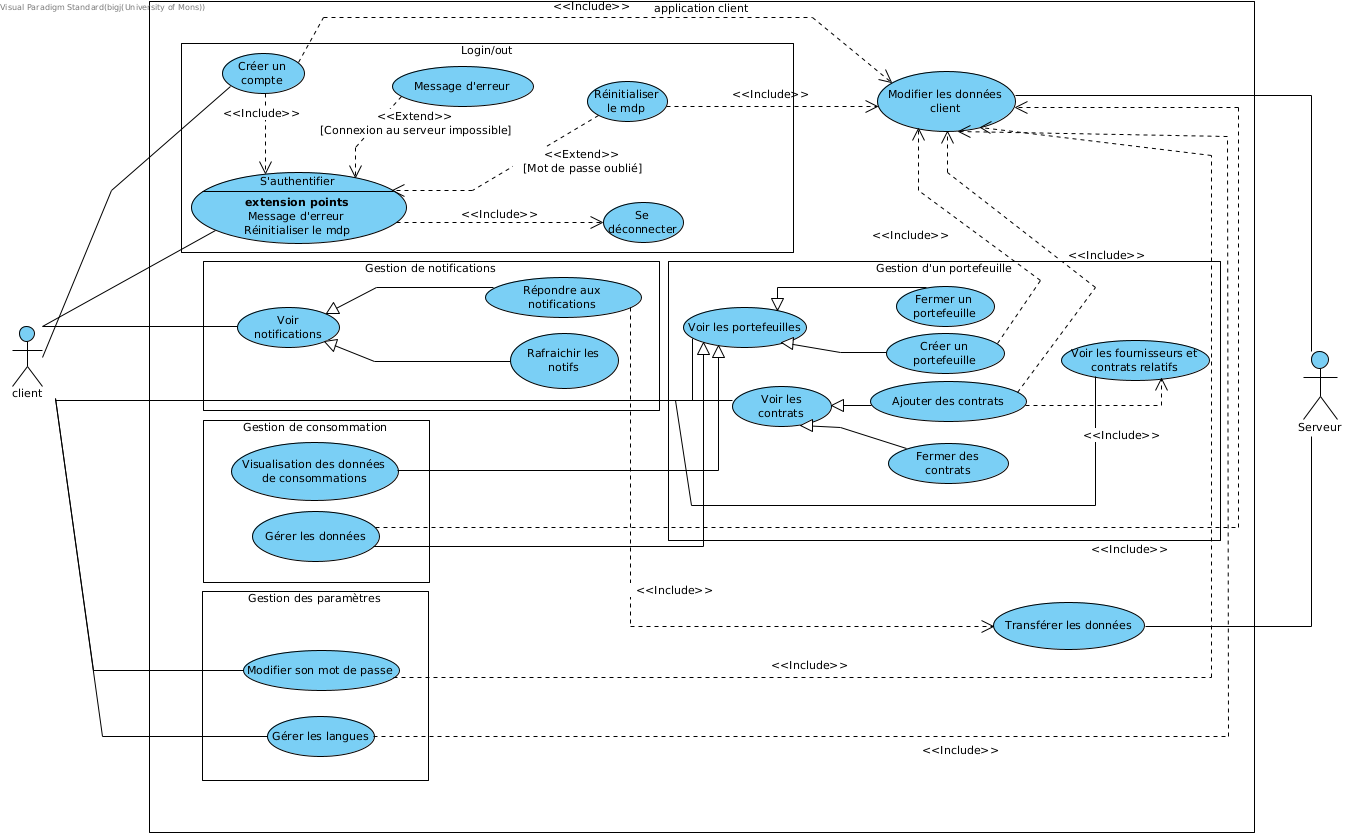
\includegraphics[width = 1\textwidth]{use_case/client.png}
\end{figure}

\subsection{Fournisseur}
	Pour le fournisseur, l'organisation des use case reste la même. 
	
\begin{figure}[h]
\centering
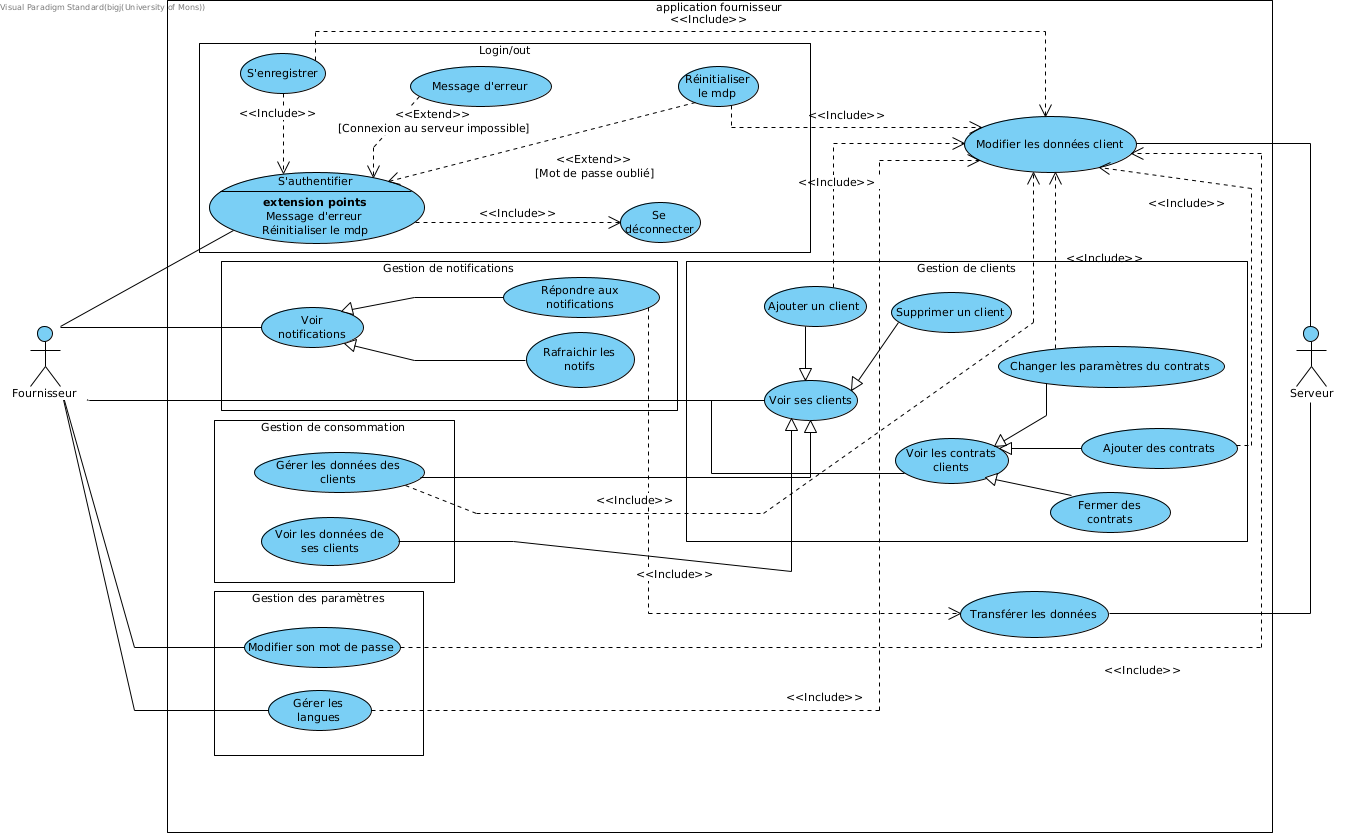
\includegraphics[width = 1\textwidth]{use_case/fournisseur.png}
\end{figure}